\documentclass[a4paper]{article}
\usepackage[pdftex]{graphicx}
\usepackage[utf8]{inputenc}
\usepackage{enumerate}
\usepackage{siunitx}
\sisetup{locale=DE} 
\usepackage{icomma}
\usepackage{amssymb}
\usepackage{tikz}
\usepackage{href-ul}
\hypersetup{
	colorlinks=true,
	linkcolor=blue,
	urlcolor=blue}
\usepackage{geometry}
\geometry{a4paper, top=15mm, left=15mm, right=15mm, bottom=15mm,
	headsep=10mm, footskip=12mm}
\hyphenation{Ge-wichts-kraft}

\begin{document}
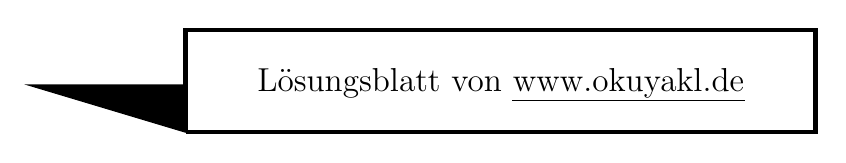
\begin{tikzpicture}(10,3)
	\draw[ultra thick](2,0) --(10,0) -- (10,1.3) --(2,1.3) -- (2,0);
	\draw[fill=black](2,0)-- (0,.6) -- (2,.6) -- (2,0);
	\node at (6,.6) {\large Lösungsblatt von \href{https://www.okuyakl.de}{www.okuyakl.de}};
\end{tikzpicture}
\vspace{0.5 cm}

\noindent{\bf Aufgabe 1. a)}\\
\begin{minipage}{0.7\textwidth}
	 Die Oberfläche eines Körpers ist immer mehr oder weniger rau. Bei Berührung zweier Körper verzahnen sich diese Rauigkeiten ineinander, und zwar umso stärker, je höher der Anpressdruck ist. Der eingekreiste Bereich in nebenstehender Skizze stellt eine Vergrößerung der Kontaktstelle dar. 
\end{minipage}
\begin{minipage}{0.3\textwidth}
	\includegraphics[width=5 cm]{reib122}
\end{minipage}
\vspace{0.5 cm}

\noindent{\bf Aufgabe 1. b)}\\
Man kann die Anpresskraft verringern, die Oberflächen durch Polieren glätten oder mit einem Gleitmittel wie Öl oder Schmierseife versehen.
\vspace{0.5 cm}

\noindent{\bf Aufgabe 1. c)}\\
Bei einem einseitigen Hebel greifen die Kräfte beide auf einer Seite vom Gelenk an; Beispiele: Nussknacker, Angelrute, Golfschläger.
\vspace{0.5 cm}

\noindent Bei einem zweiseitigen Hebel ist das Gelenk zwischen den Angriffspunkten der Kräfte; Beispiele: Zange, Schere, Wippe.
\vspace{0.5 cm}

\noindent{\bf Aufgabe 1. d)}\\
Das Drehmoment $M$ ist das Produkt aus der wirkenden Kraft $F$ mit ihrem Kraft- oder Hebelarm $a$. Wirkt eine Kraft auf einen Hebel, so bewirkt sie ein Drehmoment. Es ist umso größer, je größer $F$ und je länger $a$ ist.
\vspace{0.5 cm}

\noindent
\begin{minipage}{0.4\textwidth}
	\noindent{\bf Aufgabe 2. a)}\\
	\includegraphics[width=6 cm]{efen122}
\end{minipage}
\begin{minipage}{0.6\textwidth}
		\noindent{\bf Aufgabe 2. b)}\\
        Die Gleitreibungskraft ist proportional zu der Normalkraft $F_N$. Dies folgt aus der Tatsache, dass die Messpunkte auf einer Ursprungsgeraden liegen.
        \vspace{0.5 cm}
        
        \noindent{\bf Aufgabe 2. c)}\\
        Für die Gleitreibungszahl $\mu$ gilt:
        $$ F_G= \mu \cdot F_N$$
        Wir wählen ein Wertepaar, das auf der Geraden liegt, lösen nach $\mu$ auf und setzen ein:   
        $$ \mu = {F_G \over F_N}={\SI{0,91}{\newton} \over \SI{3,0}{\newton}}=0,30$$      
\end{minipage}
\vspace{0.5 cm}


\noindent{\bf Aufgabe 3.}\\
Es gibt sehr viele Möglichkeiten; man kann die Quader stapeln oder hintereinander legen. Die geringste Reibungszahl halt der Holzquader. Also ist die günstigste Möglichkeit, wenn der Holzquader unten liegt und die beiden anderen Quader trägt. Dann werden die Gewichte nur mit dem kleinsten $\mu$ multipliziert.
\vspace{0.5 cm}

\noindent{\bf Aufgabe 4.}\\
Die Hubarbeit ist 
$$W=F_G\cdot h \quad \Rightarrow \quad h = {W \over F_G} = {\SI{12000}{\joule} \over \SI{1500}{\newton}} = \SI{8}{\meter}$$
\vspace{0.5 cm}

\noindent{\bf Aufgabe 5.}\\
Arbeit ist Leistung mal Zeit und gleichzeitig (Reibungs-)Kraft mal Strecke:
$$ P \cdot t = \mu \cdot F_G \cdot s \quad \Rightarrow \quad F_G = {P \cdot t \over \mu \cdot s}= 
{\SI{20}{\watt} \cdot \SI{10}{\second} \over 0,20 \cdot \SI{2,0}{\meter}} = \SI{500}{\newton}$$
Einheitencheck:
$$ {\SI{}{\watt}\cdot \SI{}{\second} \over \SI{}{\meter}}= {\SI{}{\newton\meter} \over \SI{}{\meter}}=\SI{}{\newton}$$
\vspace{0.5 cm}
\begin{center}
	\includegraphics[width=7 cm]{../../viecher/endcomic.pdf}
	
	Hier geht es zurück zum \href{https://www.okuyakl.de/phys/p8reibL122/aa122.pdf}{Aufgabenblatt}
\end{center}

\end{document}